\documentclass[letterpaper]{article}
\usepackage[utf8]{inputenc}
\usepackage[margin=0.9in]{geometry}
\usepackage{pdfpages}
\usepackage{xcolor}
\usepackage{helvet}
\renewcommand{\familydefault}{\sfdefault}
\usepackage{hyperref}
\usepackage{bookmark}
\hypersetup{
  pdftitle={Hanzo --- Technical Paper Compendium},
  pdfauthor={Hanzo AI Research --- Hanzo Industries},
  colorlinks=true, linkcolor=black, urlcolor=black,
  bookmarksopen=true, bookmarksnumbered=false}
\setlength{\parindent}{0pt}

\begin{document}

% ---- Clickable contents page (internal links — work with no website) -------
\thispagestyle{empty}
{\Large\bfseries Hanzo --- Technical Paper Compendium}\\[2pt]
{\large Sovereign AI, Post-Quantum, FHE \& Agentic Engineering}\\[1.5em]
{\footnotesize\color{gray}Owned, self-hostable AI and cryptography for regulated industries, critical
infrastructure, and government. Click any title to jump to the paper; the PDF bookmark sidebar also navigates
the suite. The full suite is published at papers.hanzo.ai.}\\[1.5em]

\textbf{Start here}\\[0.4em]
\begin{tabular}{@{}p{0.96\linewidth}@{}}
\hyperref[c00]{Overview --- Hanzo Cloud for Reindustrialization (one-pager)}\\[0.3em]
\hyperref[c01]{hanzo.ai vs.\ claude.ai --- owned AI vs.\ metered cloud}\\[0.3em]
\hyperref[c02]{Agentic Engineering at Regulated Scale}\\[0.3em]
\hyperref[c03]{Cloud Economics --- the migration case study}\\[0.3em]
\hyperref[c04]{Confidential Computing by Default (FHE)}\\[0.3em]
\hyperref[c05]{Hanzo AI for Security}\\[0.3em]
\hyperref[c06]{Hanzo AI for Compliance}\\[0.8em]
\end{tabular}

\textbf{Capability \& mission depth}\\[0.4em]
\begin{tabular}{@{}p{0.96\linewidth}@{}}
\hyperref[c07]{ZAP Protocol --- zero-copy post-quantum transport}\\[0.3em]
\hyperref[c08]{Full-Spectrum Cyber}\\[0.3em]
\hyperref[c09]{Formal Verification}\\[0.3em]
\hyperref[c10]{Autonomous Agentic AI}\\[0.3em]
\hyperref[c11]{Edge AI/ML}\\[0.3em]
\hyperref[c12]{FHE Cross-Domain}\\[0.3em]
\hyperref[c13]{Assured Networking}\\[0.3em]
\hyperref[c14]{Counter-Exploitation}\\[0.3em]
\hyperref[c15]{Quantum Sensing and QKD}\\[0.3em]
\hyperref[c16]{Test and Evaluation (V\&V)}\\[0.3em]
\end{tabular}

\vfill
{\footnotesize\color{gray}Hanzo Industries --- American-owned applied-AI lab, Techstars~'17, founded 2014.
research@hanzo.ai \quad papers.hanzo.ai}
\newpage

% ---- The suite (each entry: PDF bookmark + internal anchor label) -----------
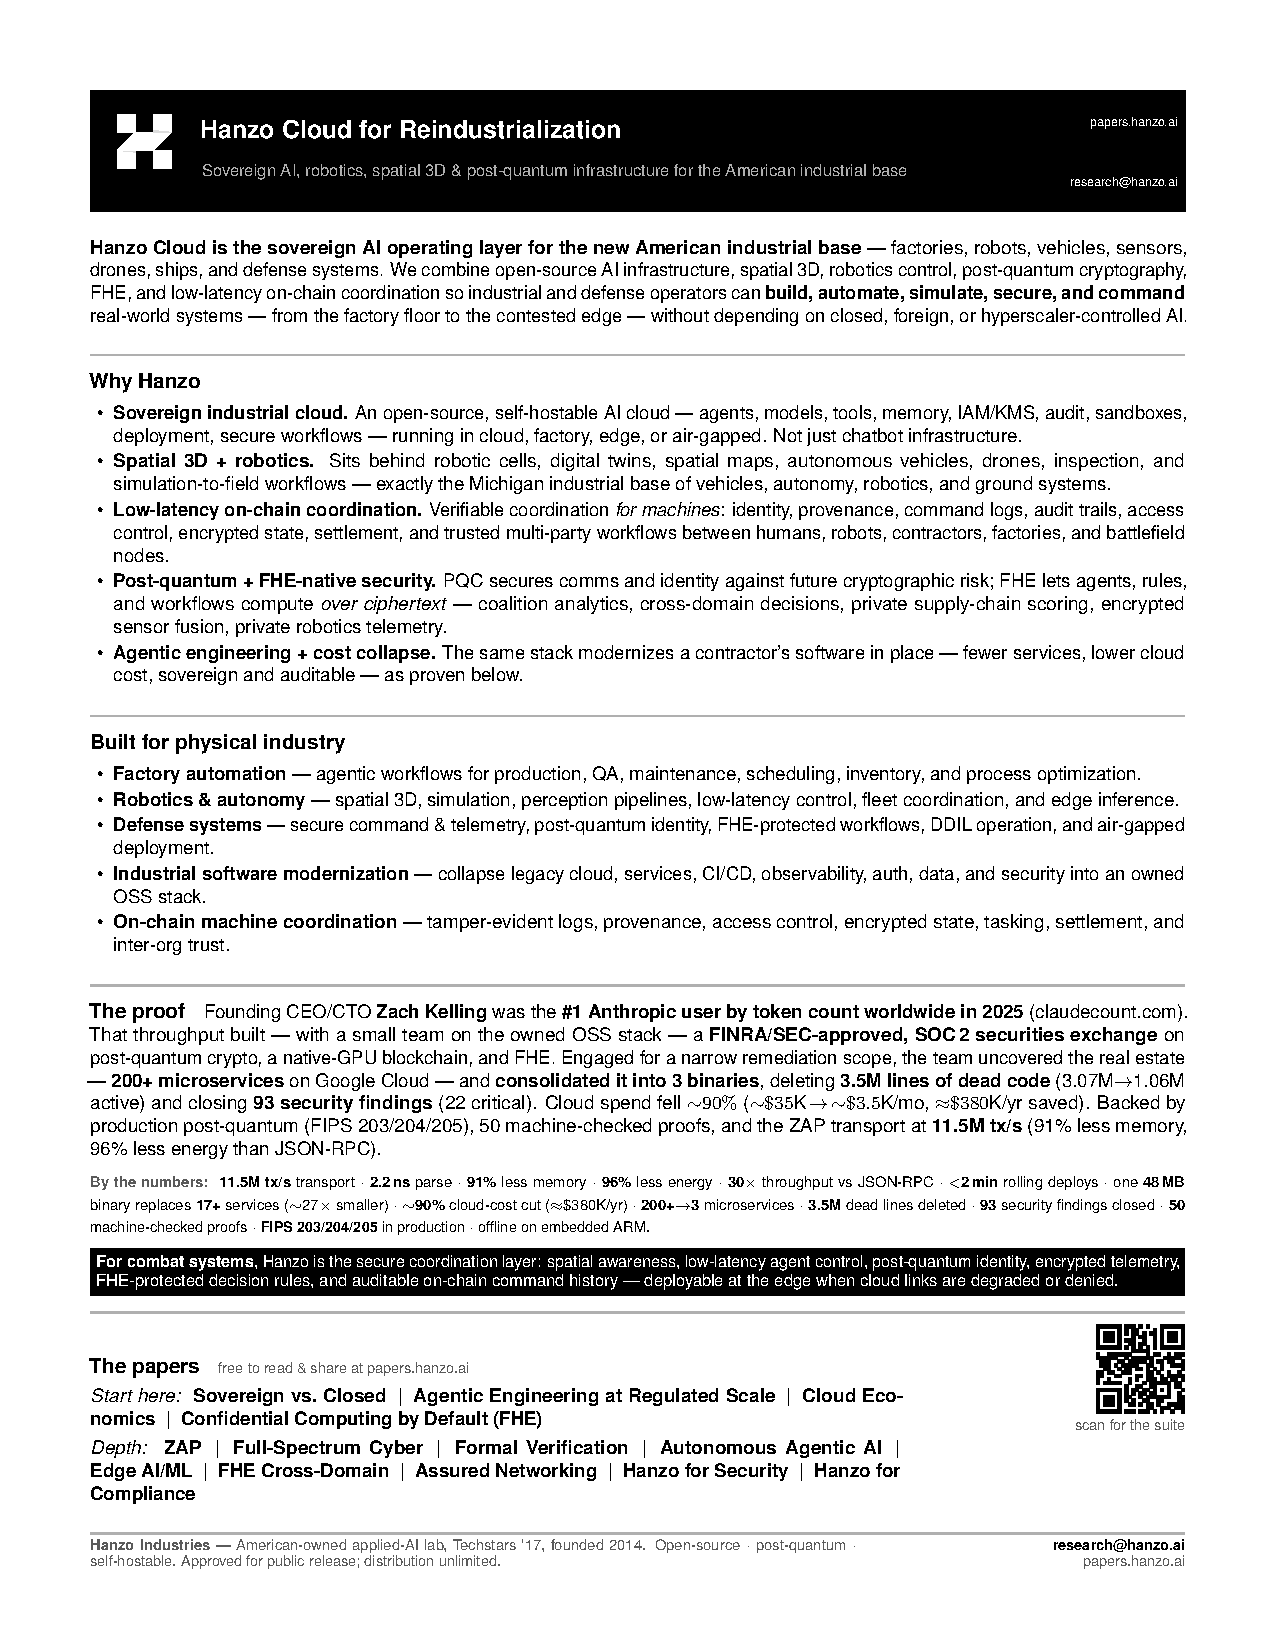
\includepdf[pages=-,fitpaper=true,addtotoc={1,section,0,{Overview: Hanzo Cloud for Reindustrialization},c00}]{hanzo-overview.pdf}
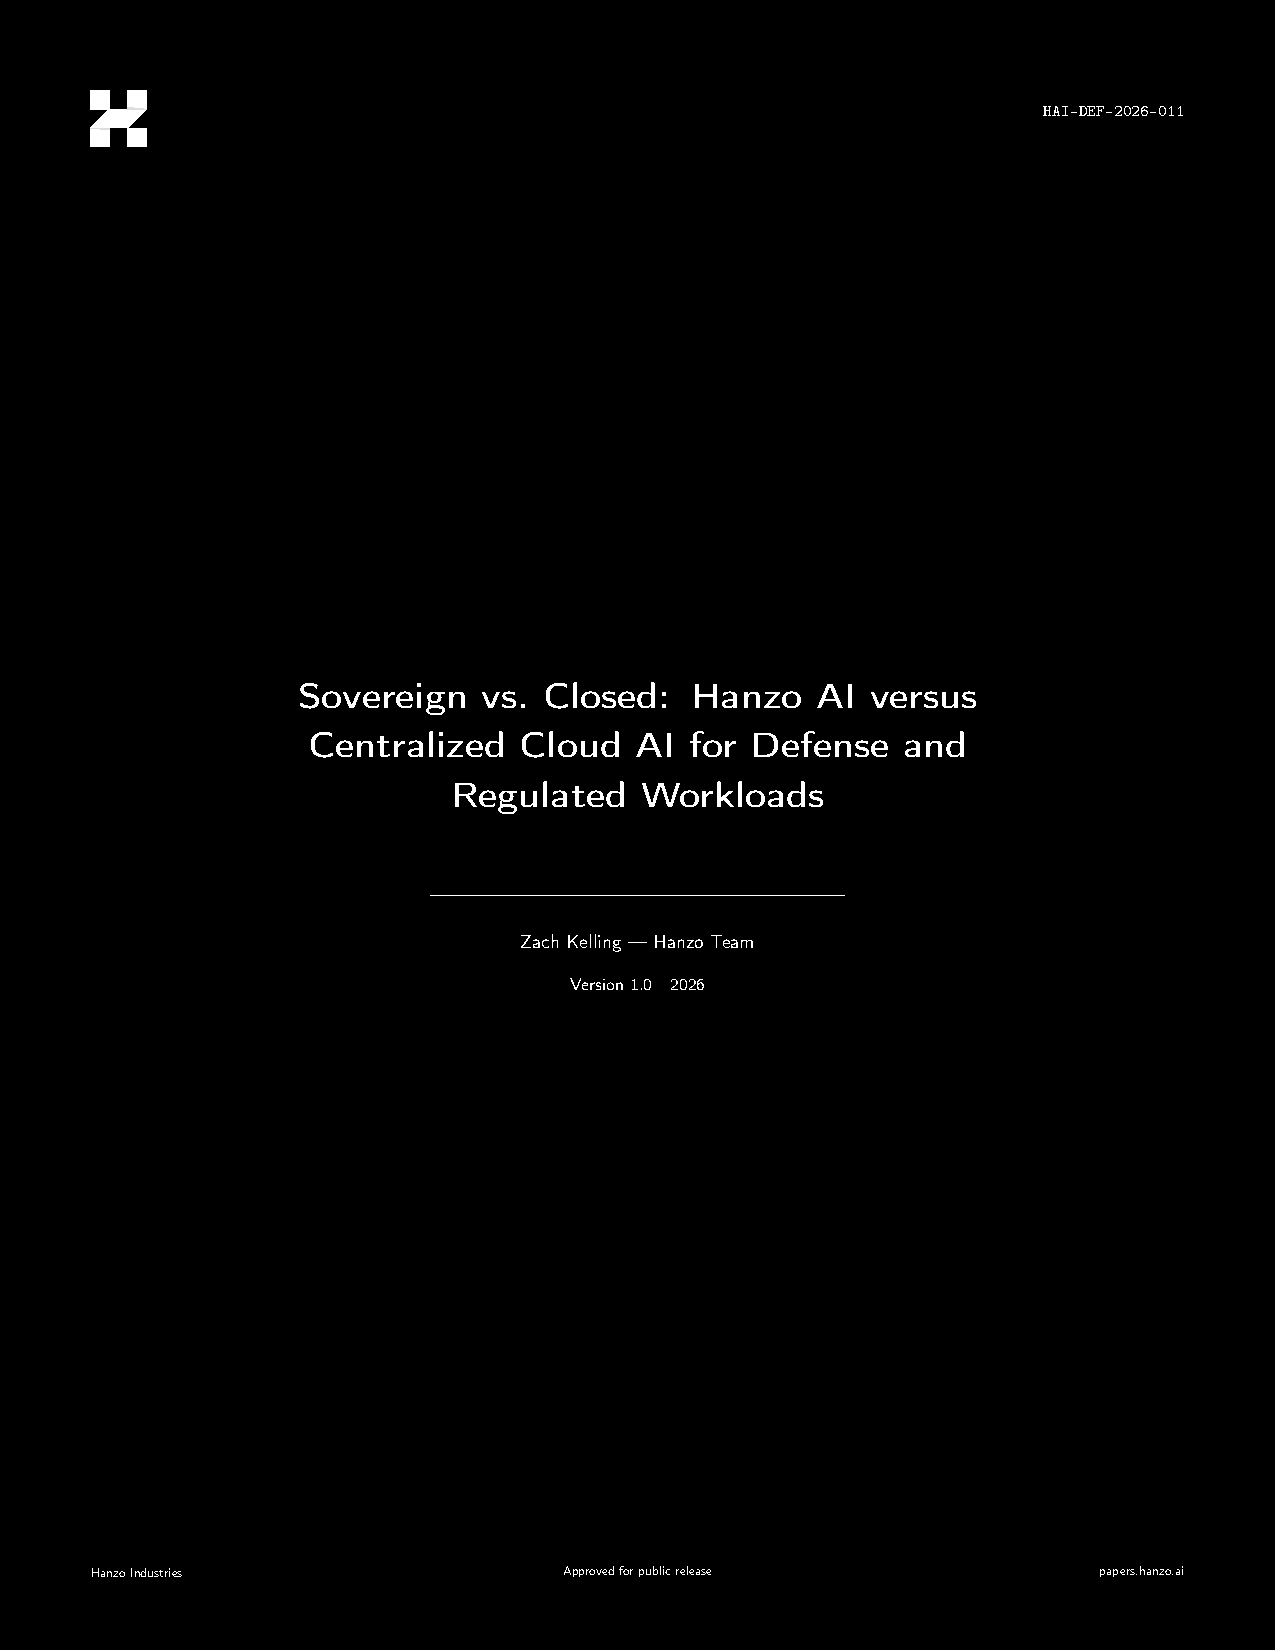
\includepdf[pages=-,fitpaper=true,addtotoc={1,section,0,{hanzo.ai vs. claude.ai},c01}]{hanzo-vs-claude.pdf}
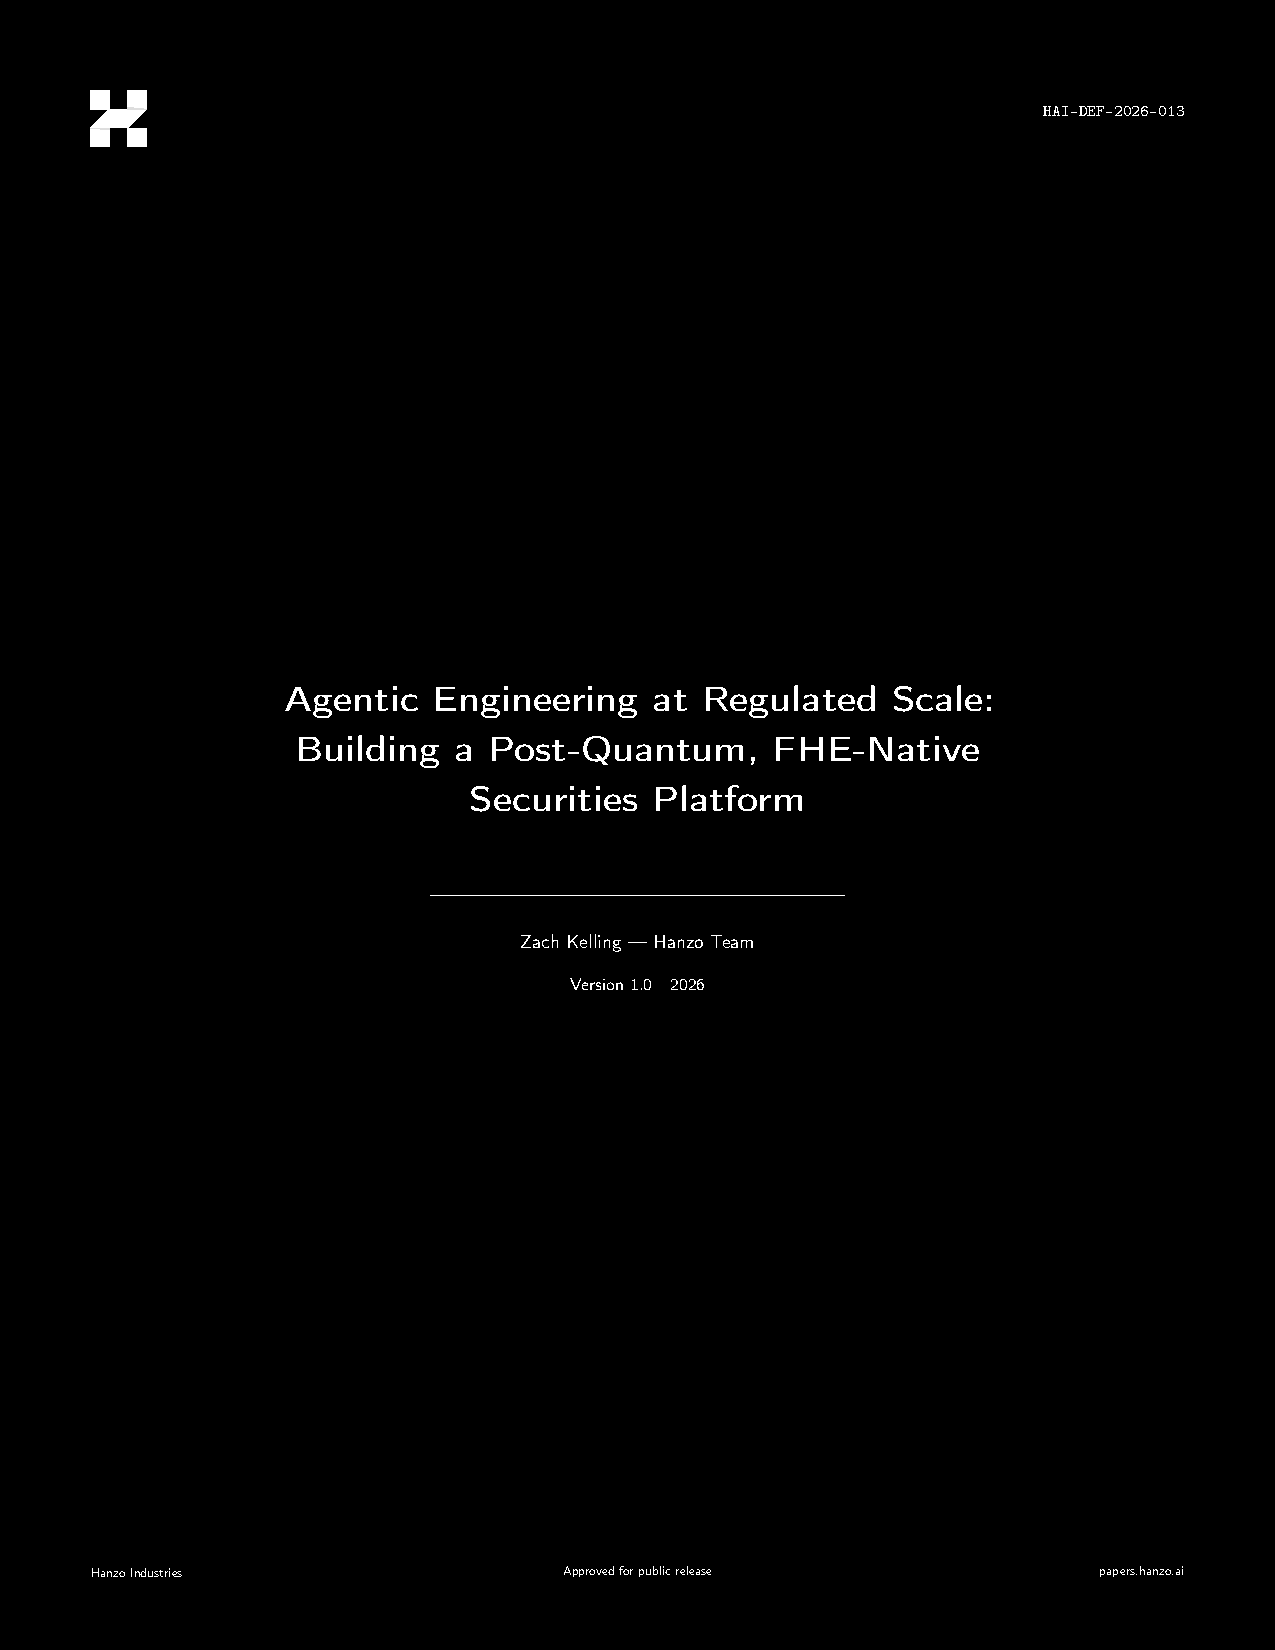
\includepdf[pages=-,fitpaper=true,addtotoc={1,section,0,{Agentic Engineering at Regulated Scale},c02}]{hanzo-agentic-prowess.pdf}
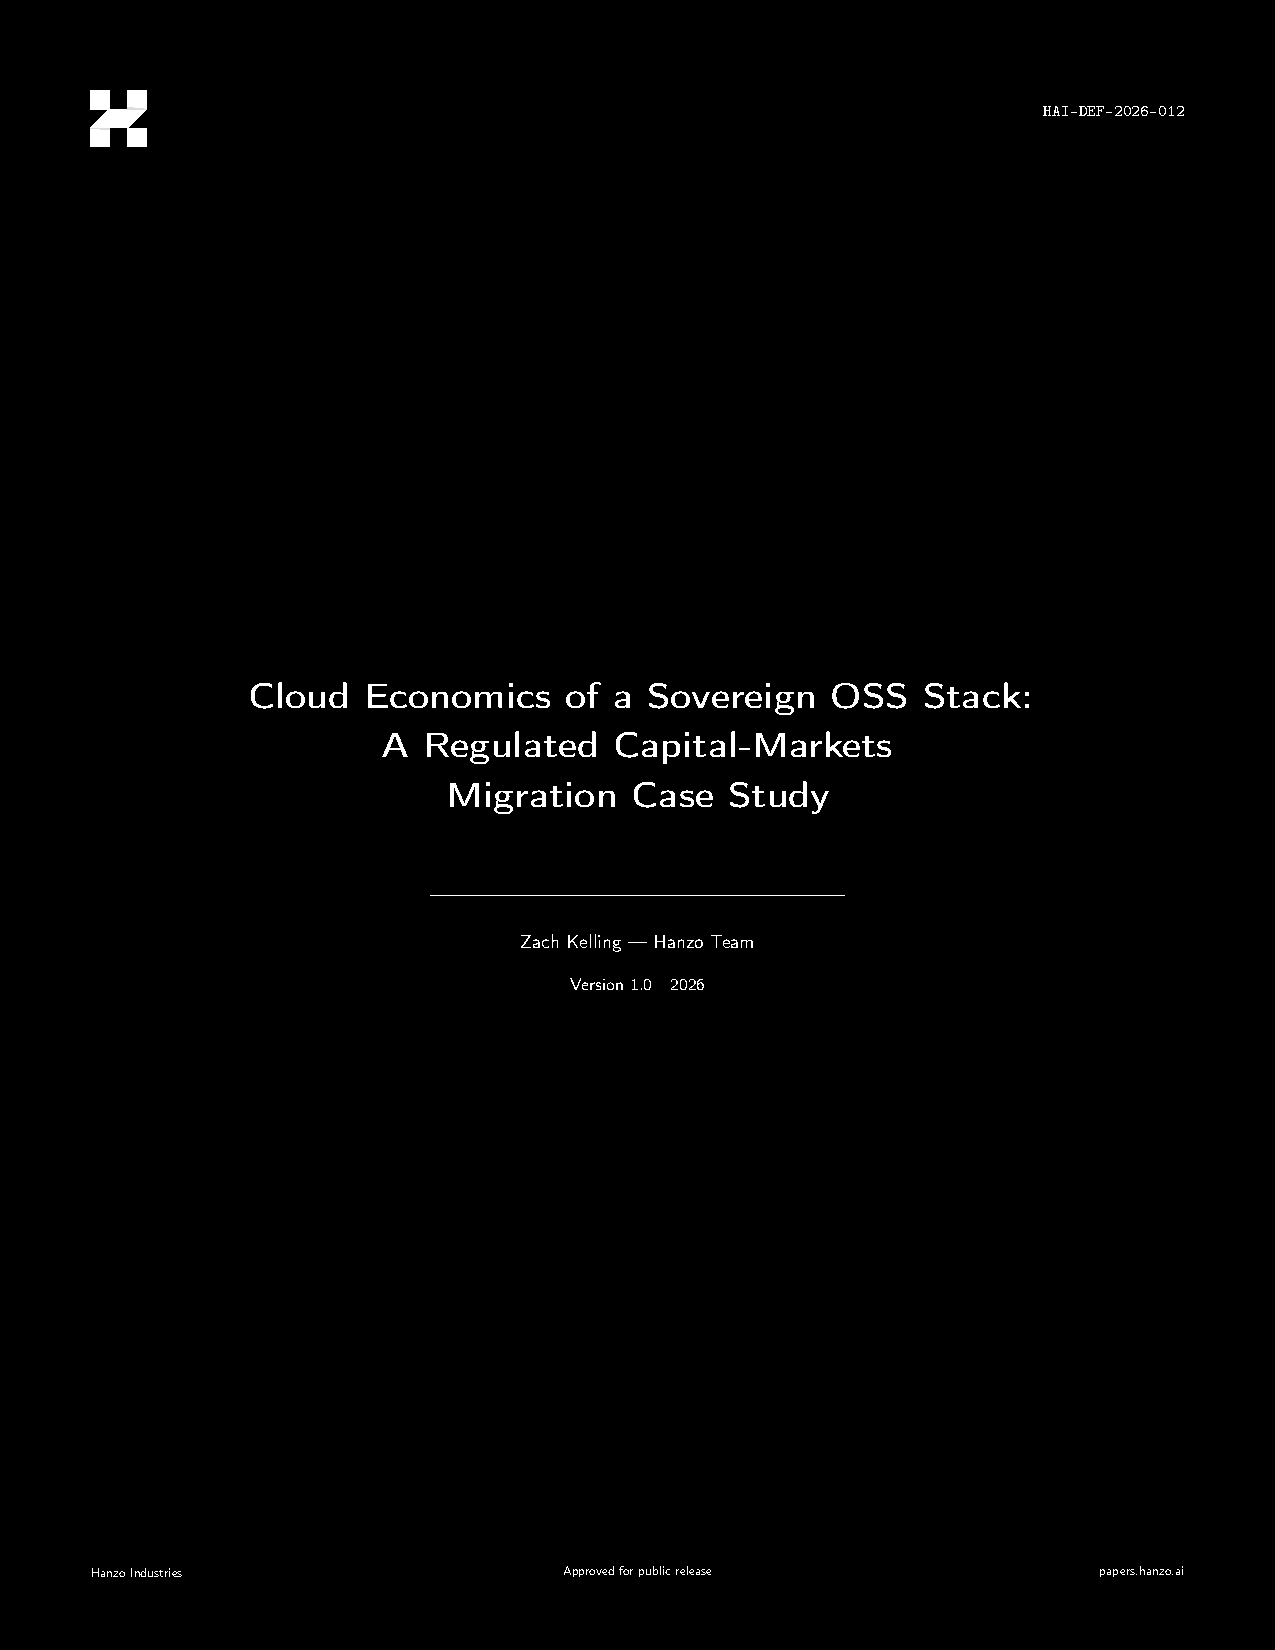
\includepdf[pages=-,fitpaper=true,addtotoc={1,section,0,{Cloud Economics: Migration Case Study},c03}]{hanzo-cloud-economics.pdf}
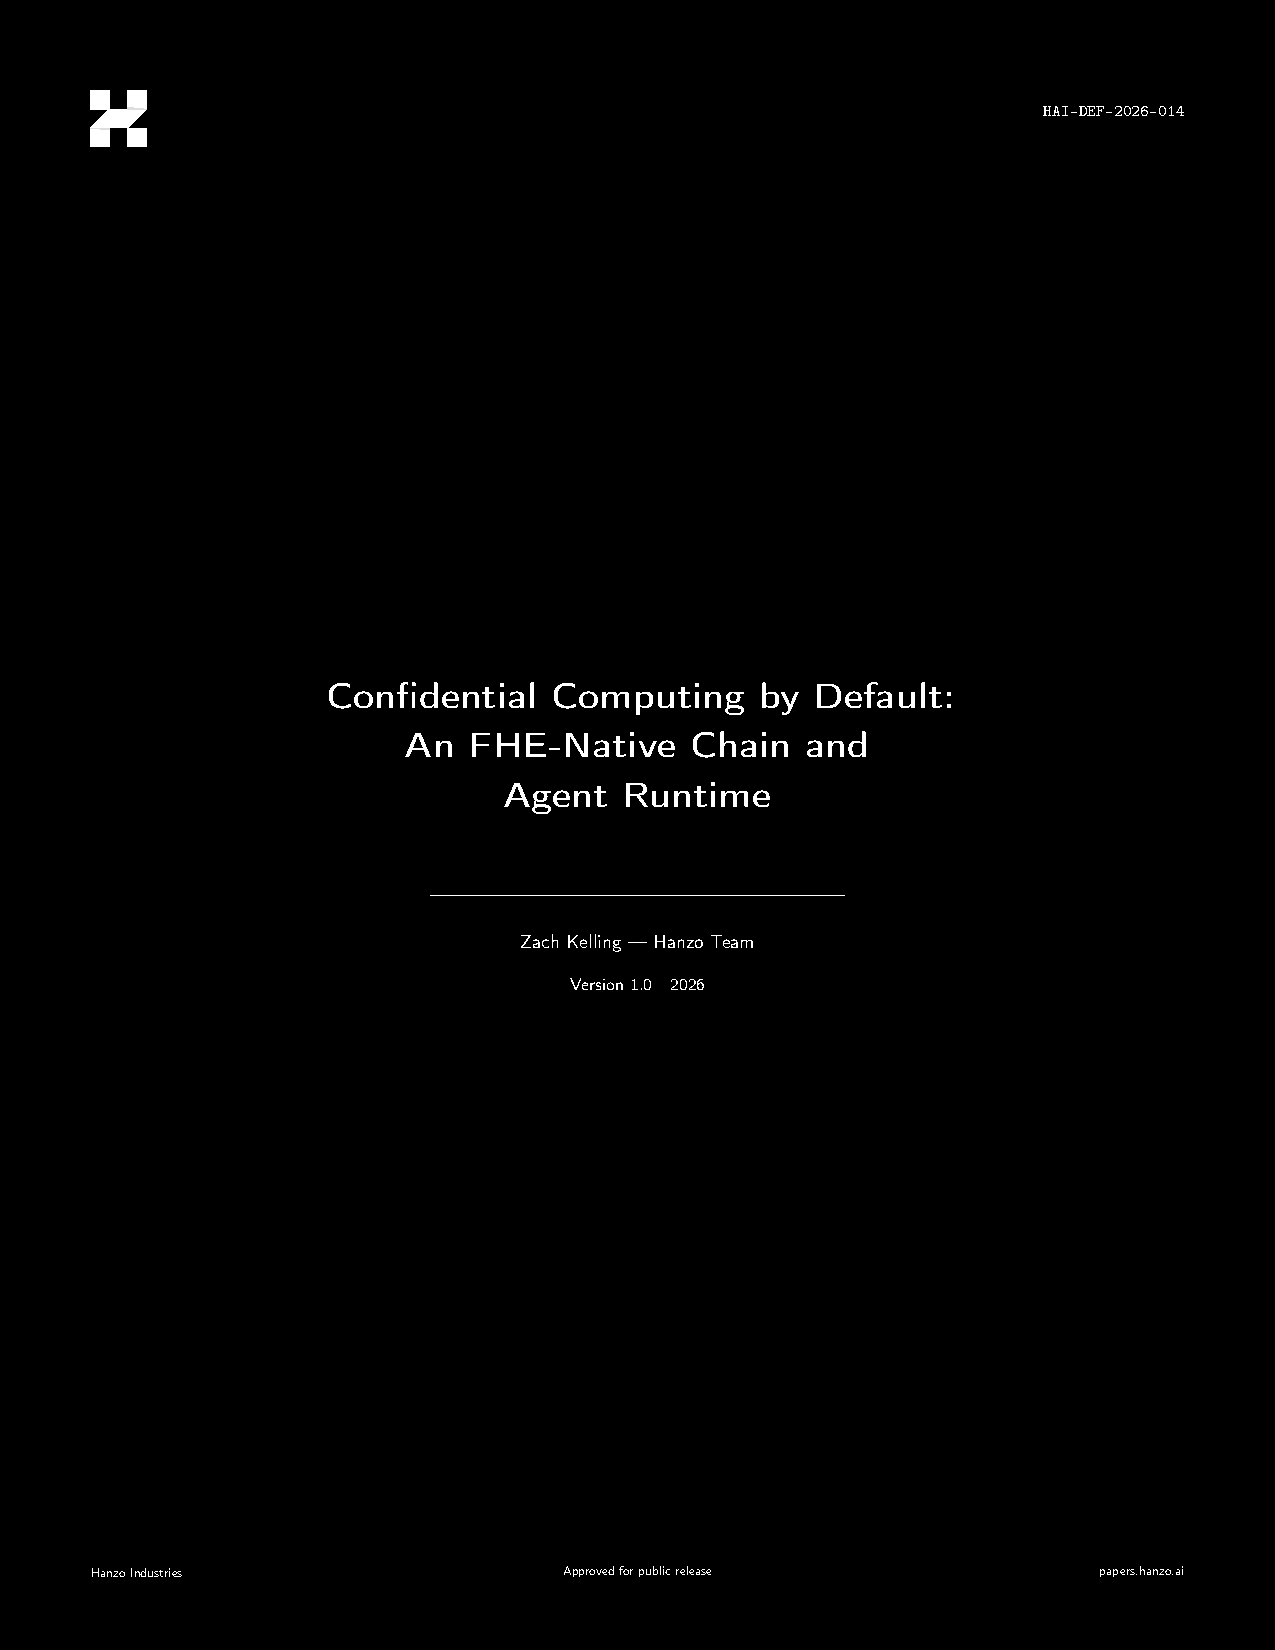
\includepdf[pages=-,fitpaper=true,addtotoc={1,section,0,{Confidential Computing by Default (FHE)},c04}]{hanzo-fhe-native.pdf}
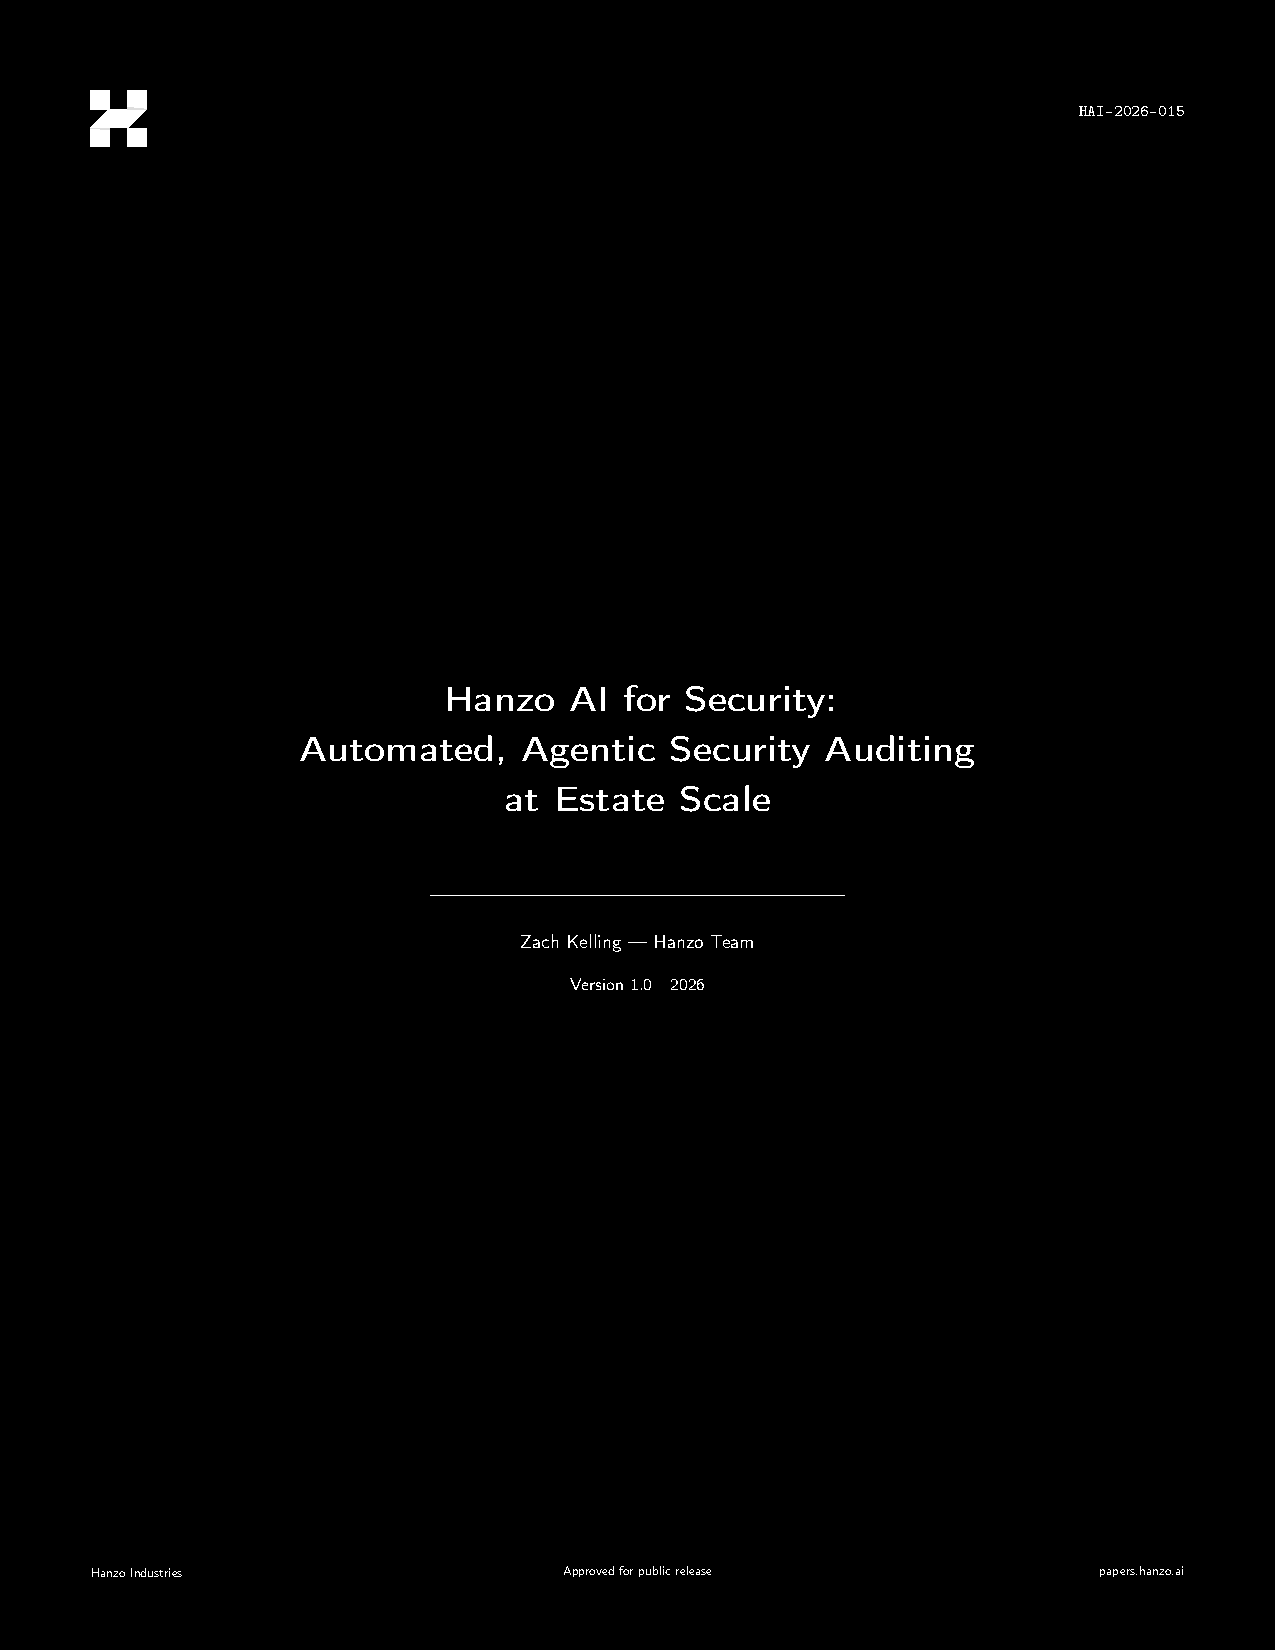
\includepdf[pages=-,fitpaper=true,addtotoc={1,section,0,{Hanzo AI for Security},c05}]{hanzo-security.pdf}
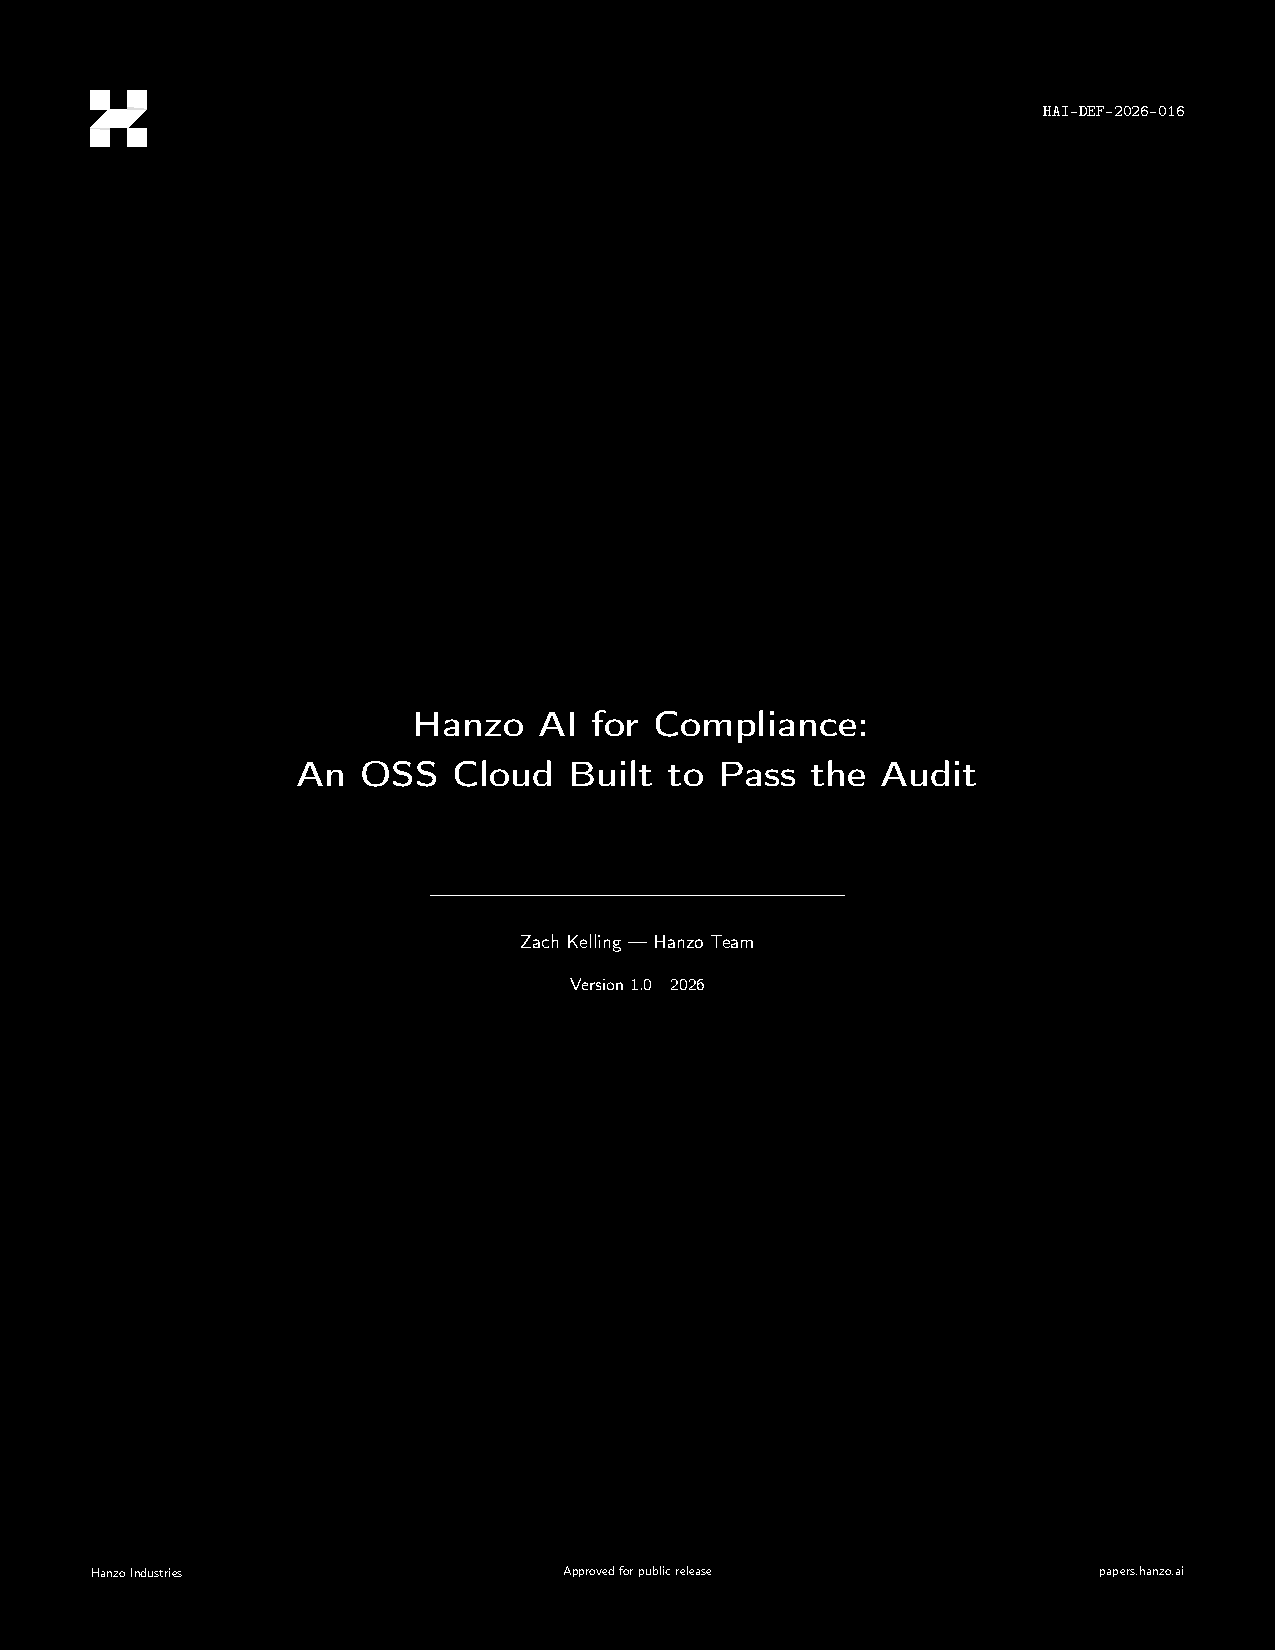
\includepdf[pages=-,fitpaper=true,addtotoc={1,section,0,{Hanzo AI for Compliance},c06}]{hanzo-compliance.pdf}
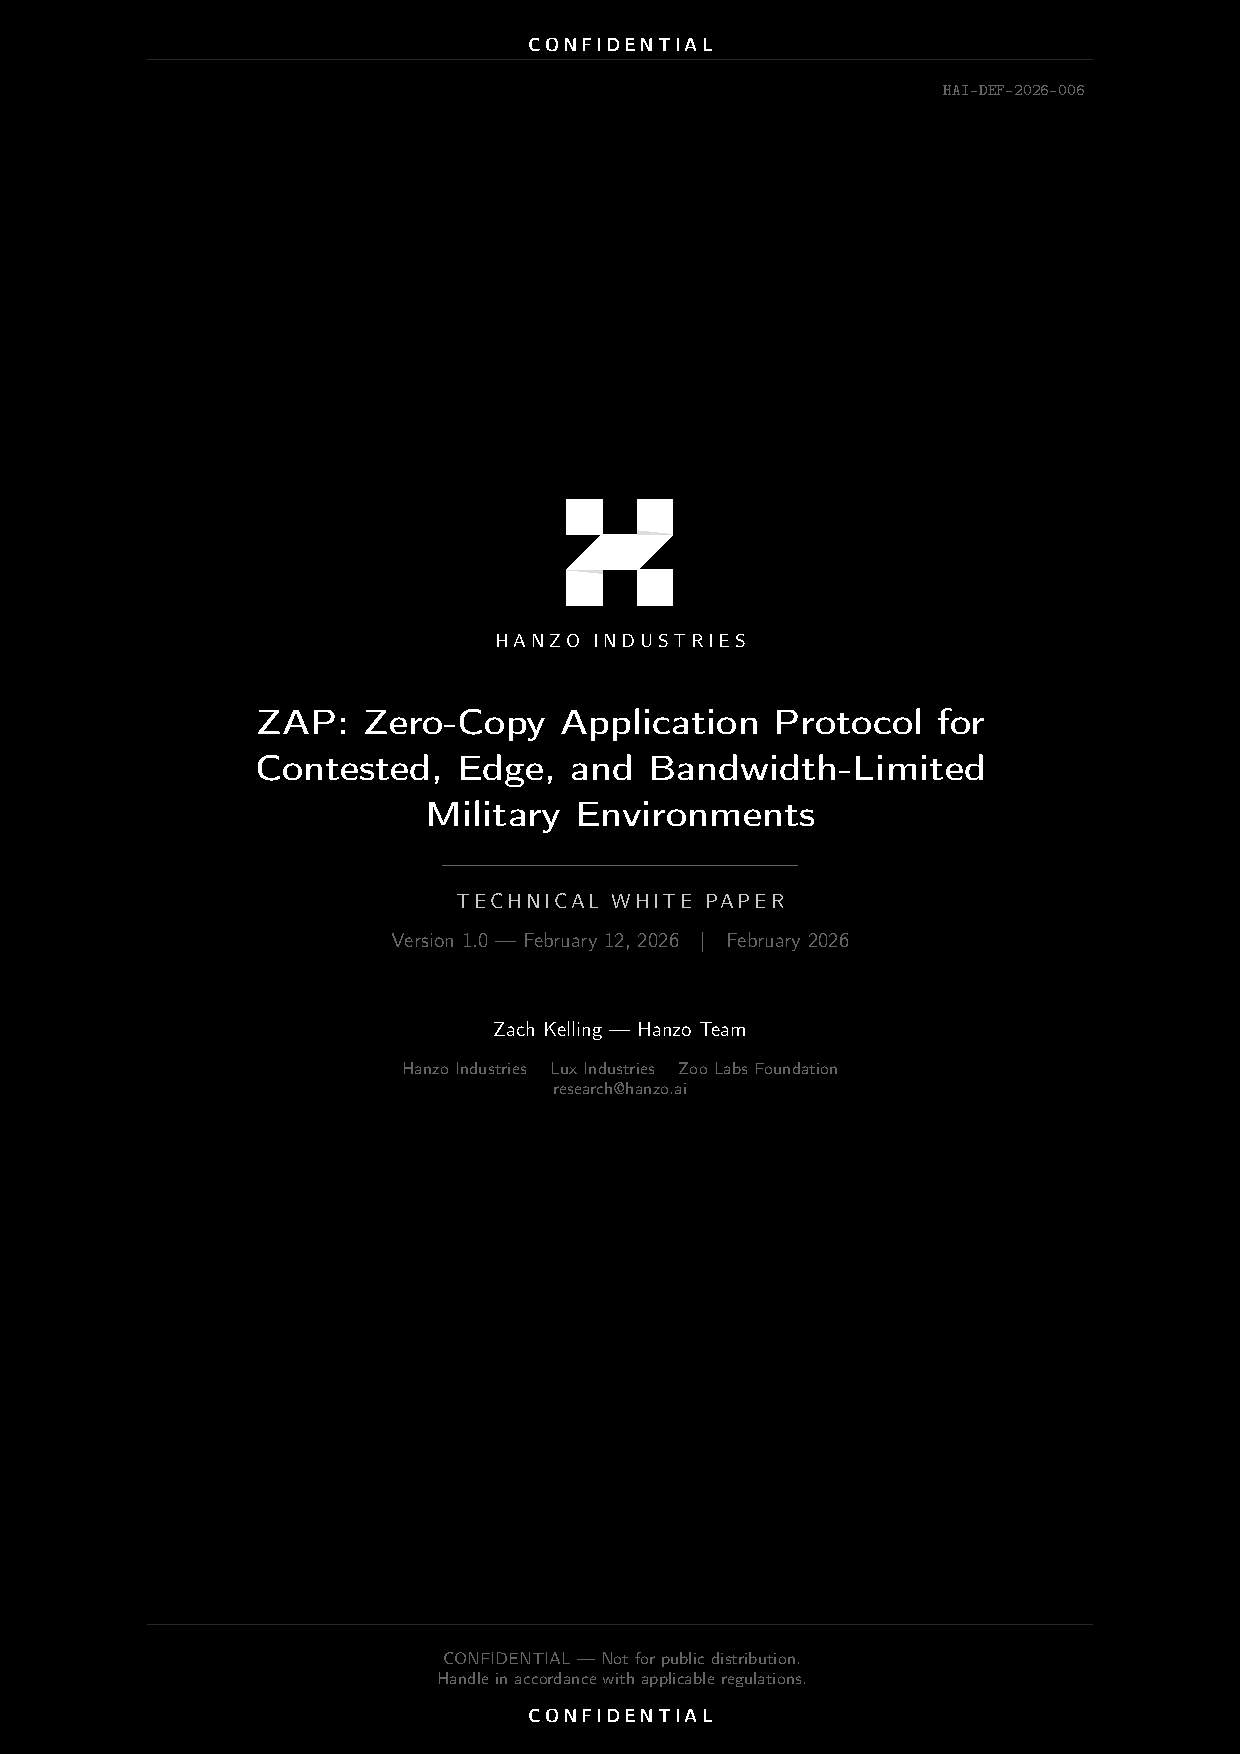
\includepdf[pages=-,fitpaper=true,addtotoc={1,section,0,{ZAP Protocol},c07}]{hanzo-zap-protocol.pdf}
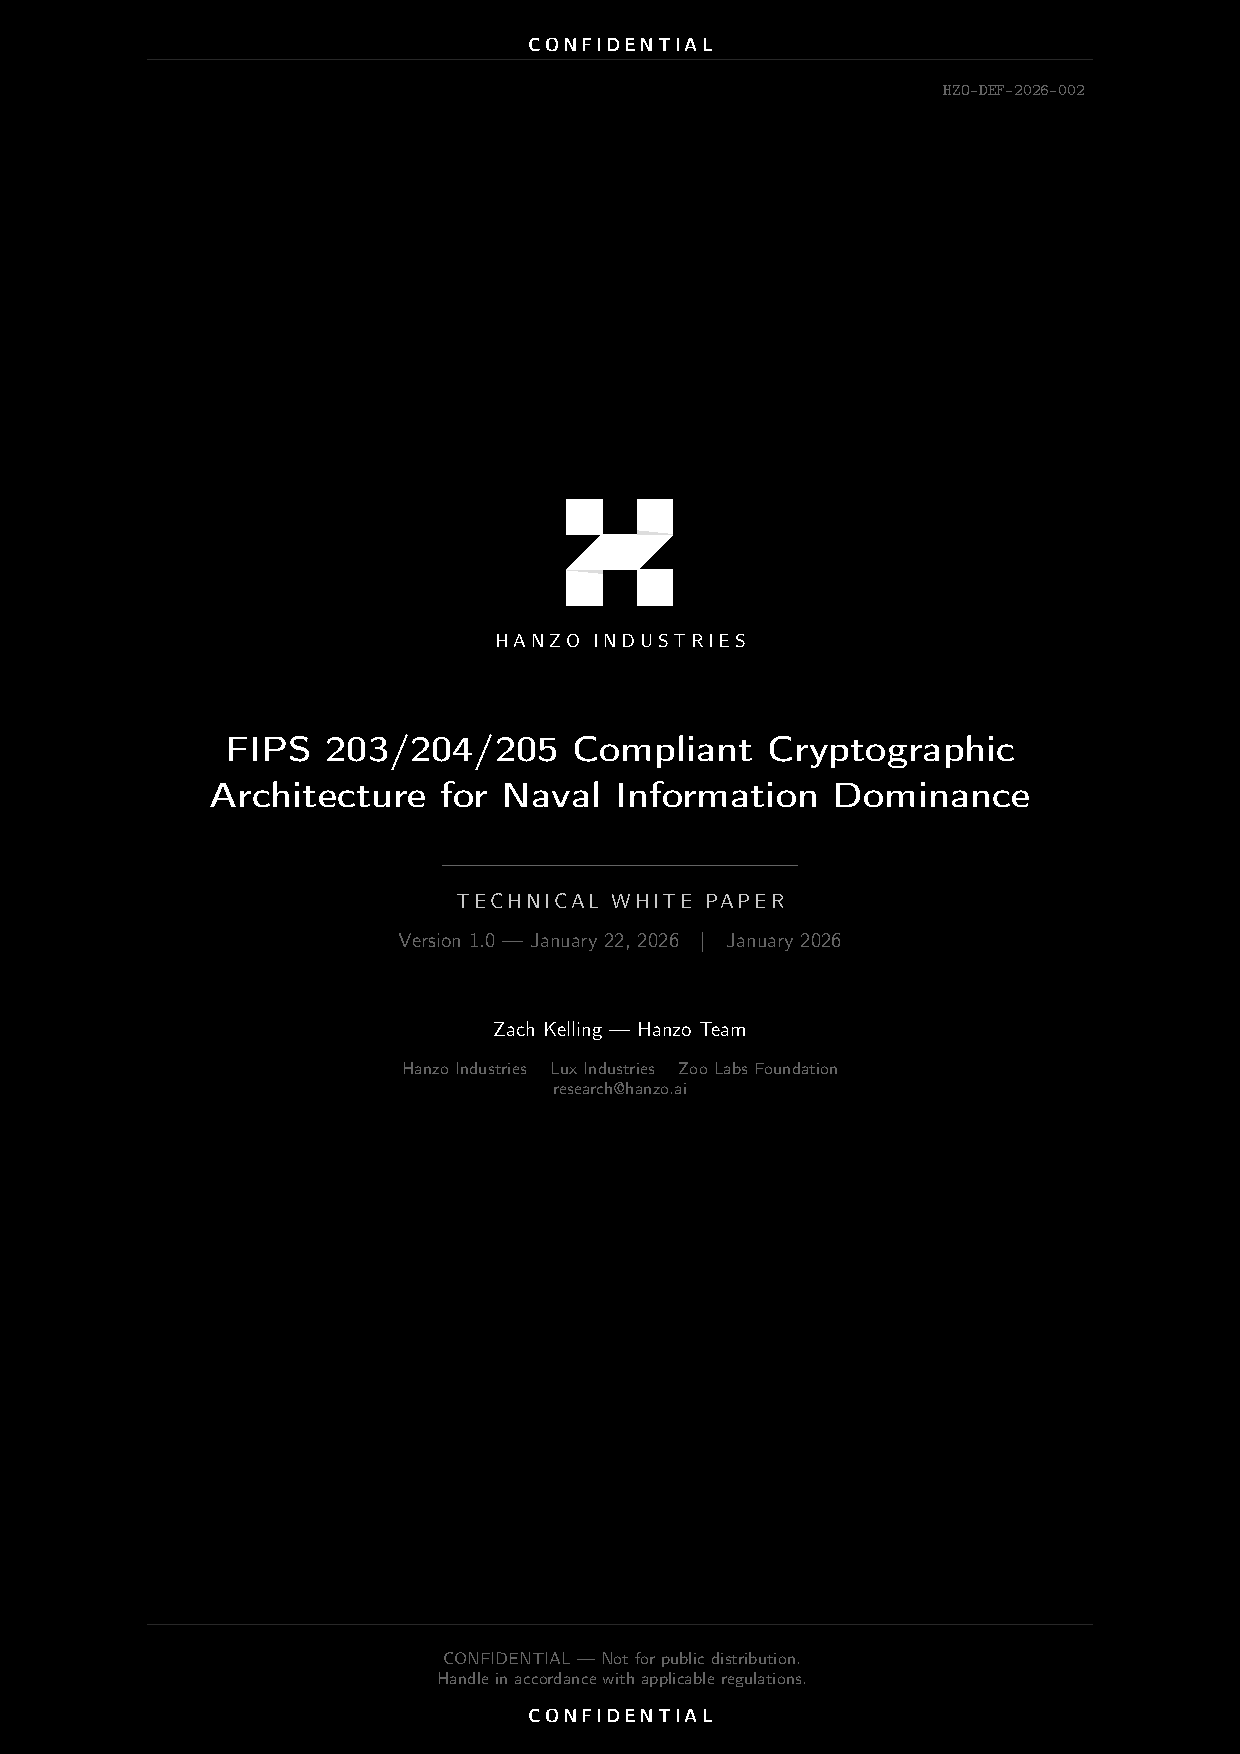
\includepdf[pages=-,fitpaper=true,addtotoc={1,section,0,{Full-Spectrum Cyber},c08}]{hanzo-full-spectrum-cyber.pdf}
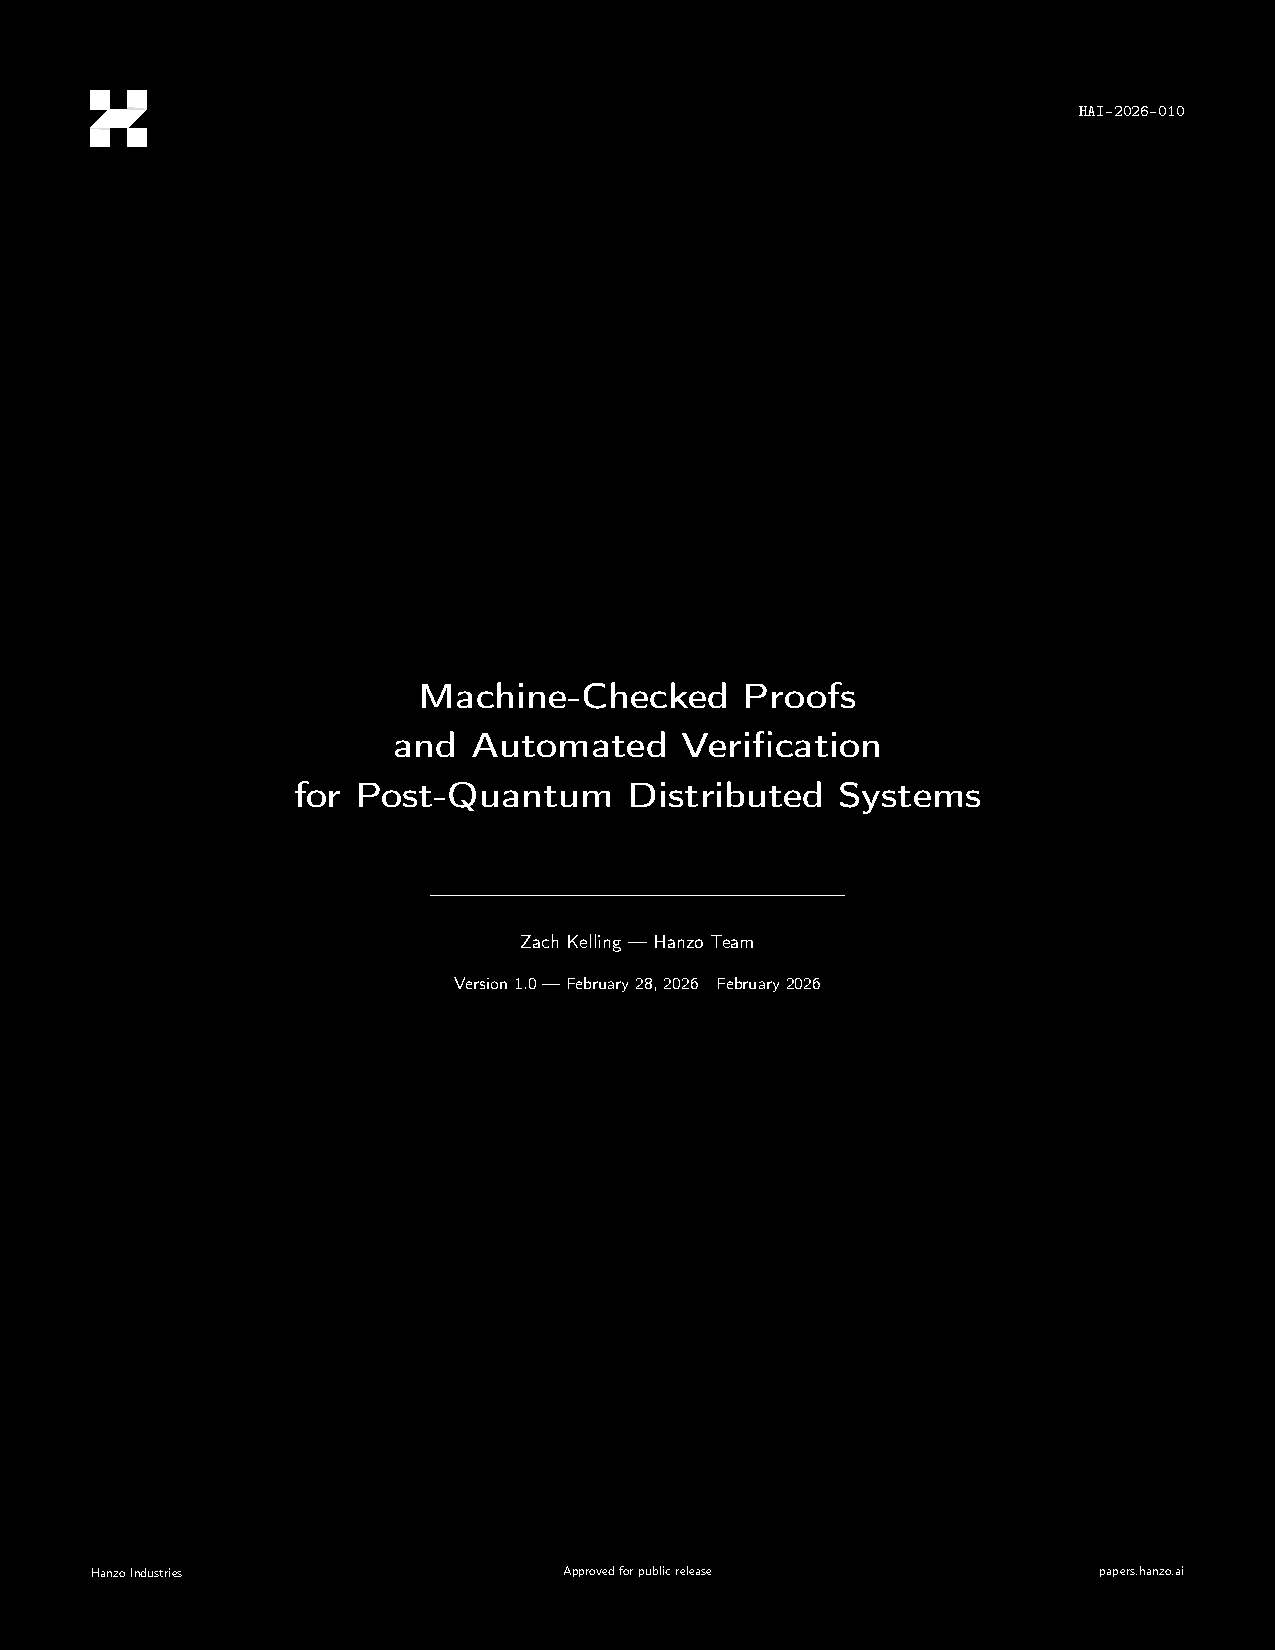
\includepdf[pages=-,fitpaper=true,addtotoc={1,section,0,{Formal Verification},c09}]{hanzo-formal-verification.pdf}
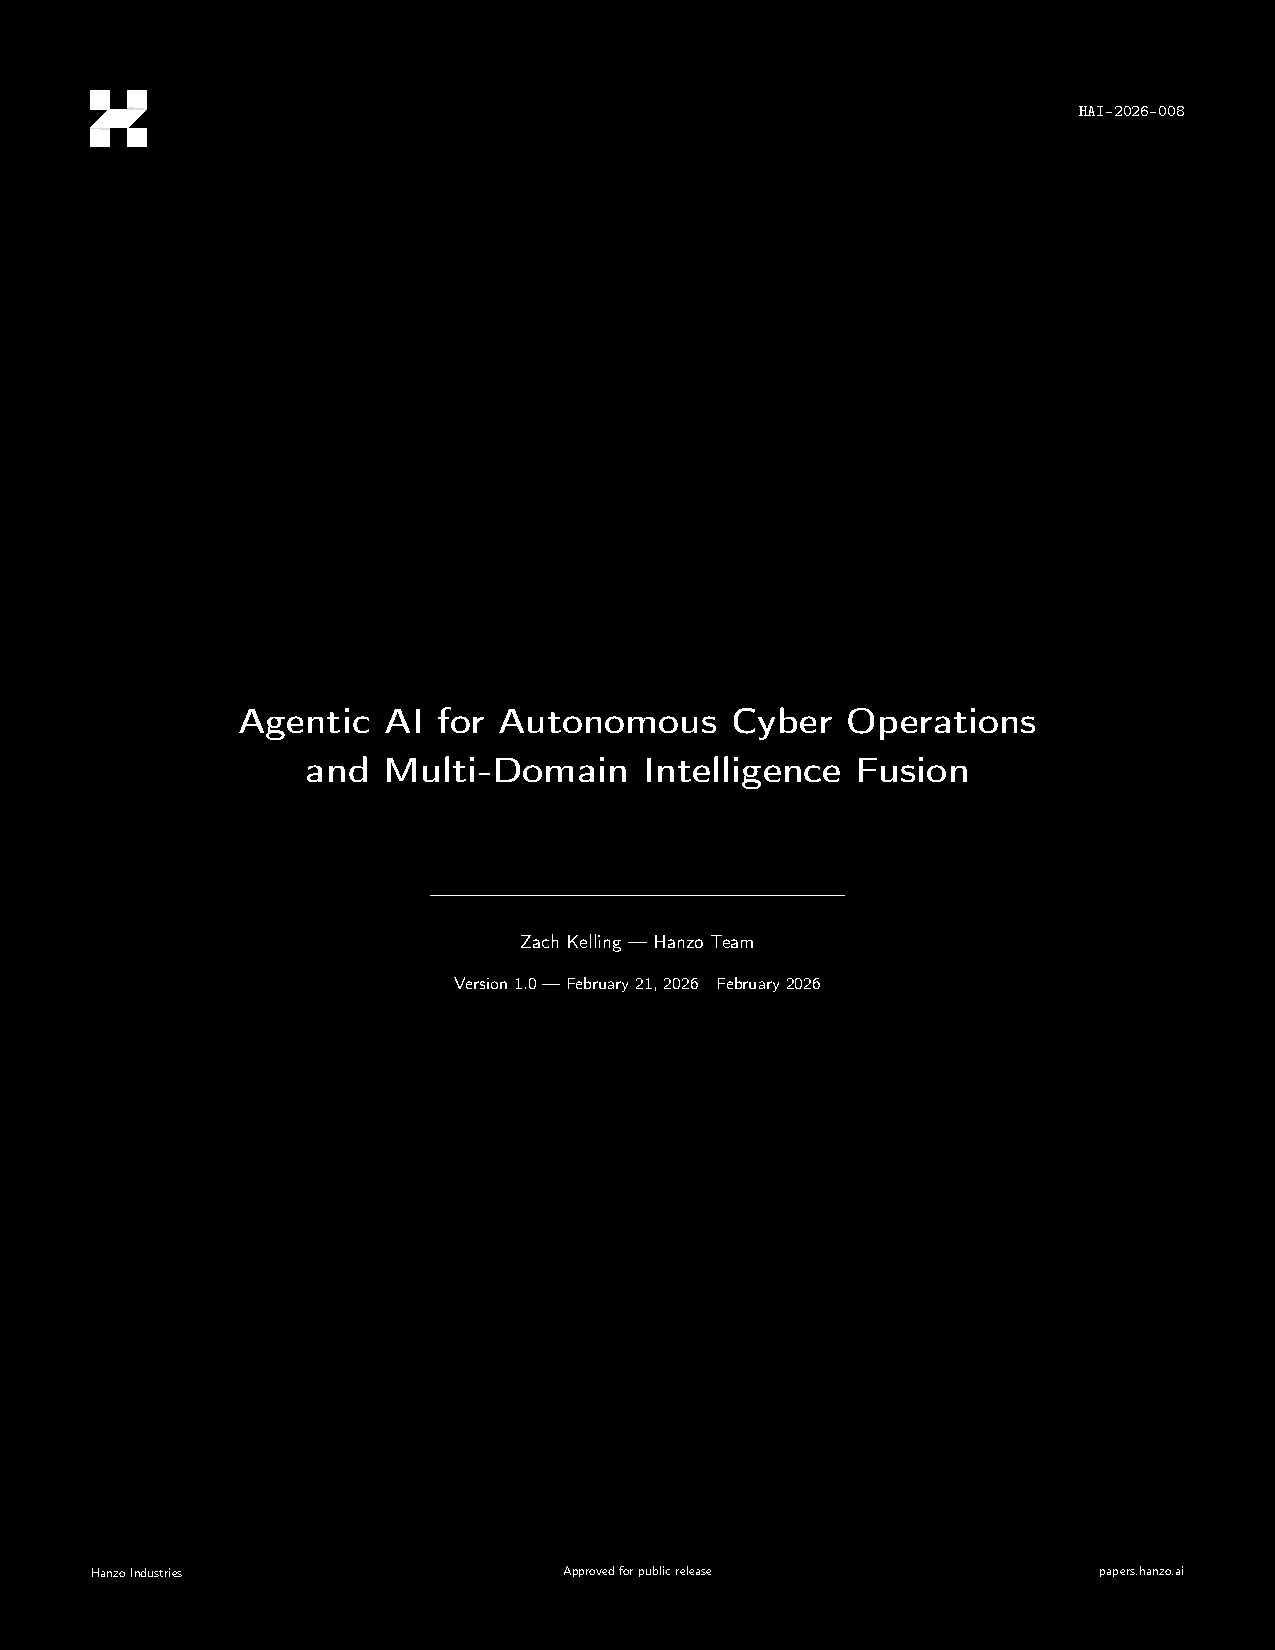
\includepdf[pages=-,fitpaper=true,addtotoc={1,section,0,{Autonomous Agentic AI},c10}]{hanzo-agentic-ai.pdf}
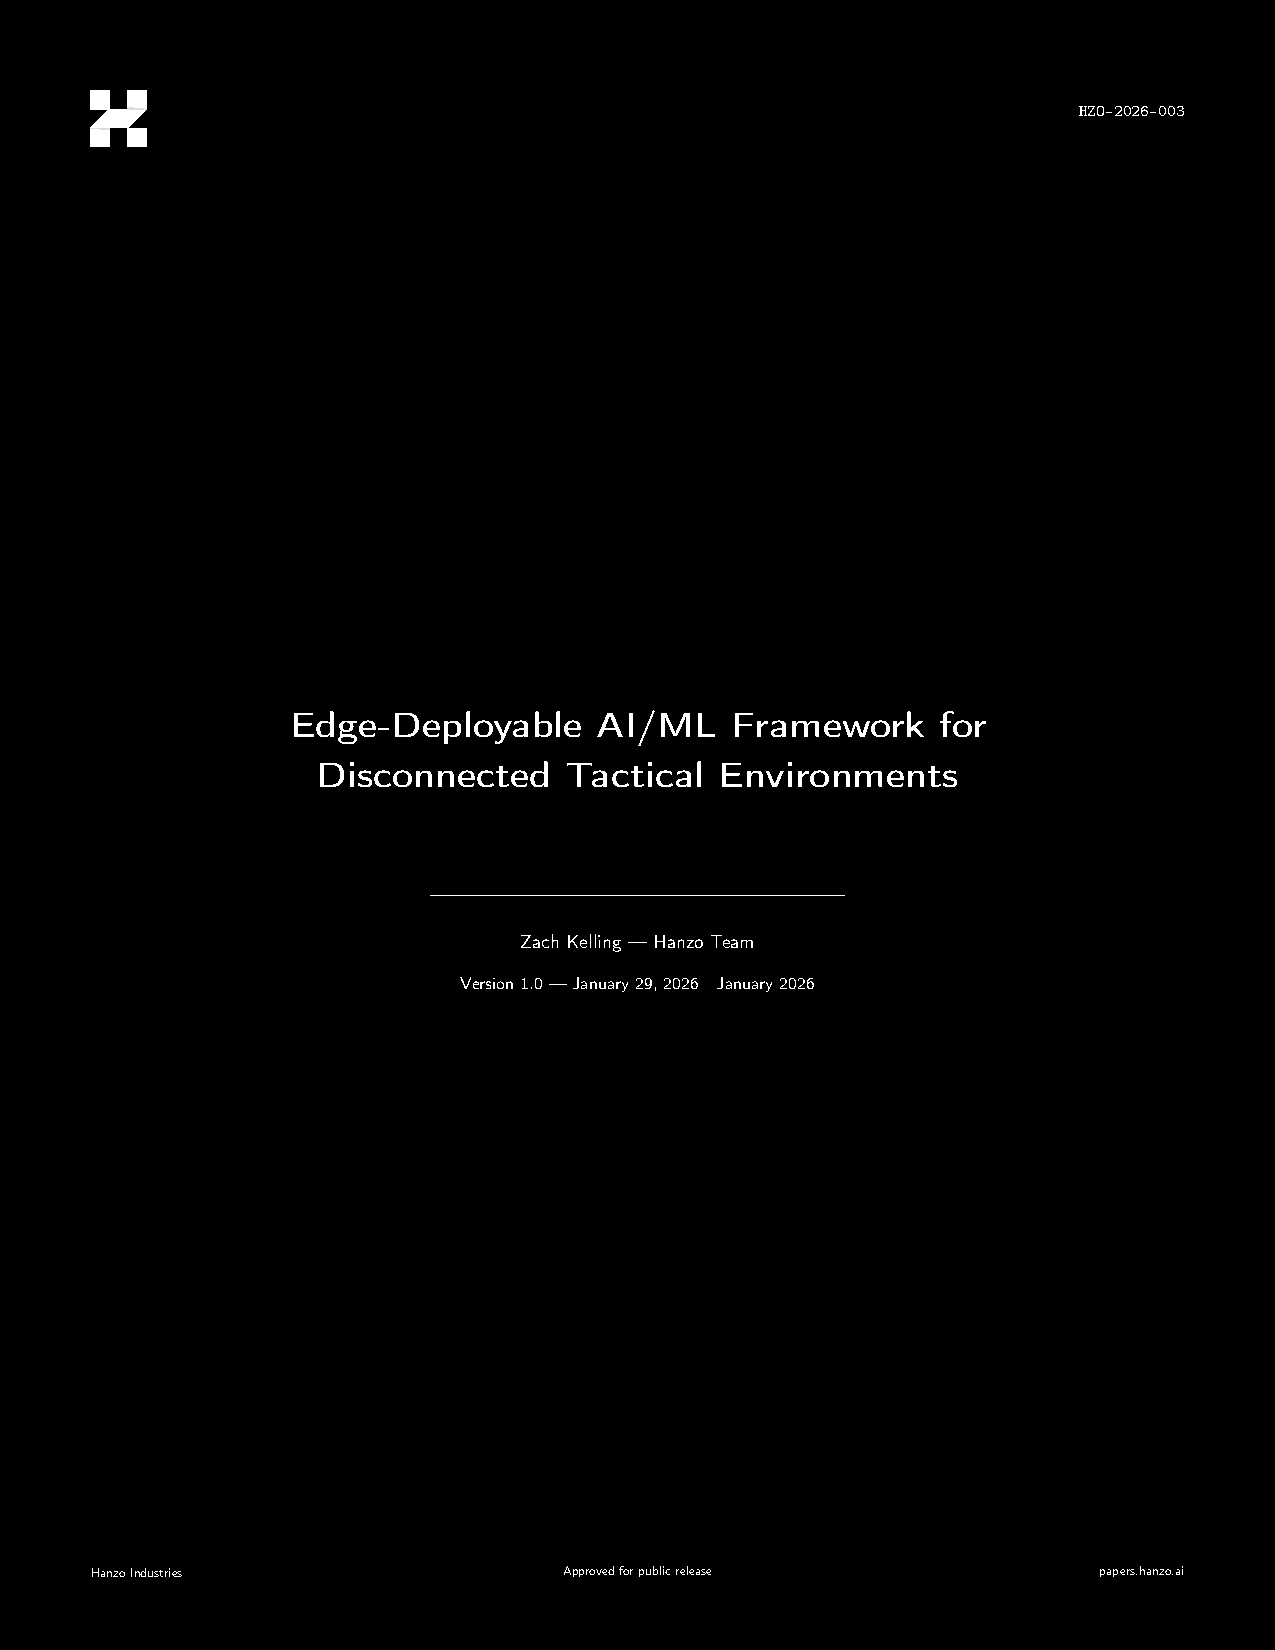
\includepdf[pages=-,fitpaper=true,addtotoc={1,section,0,{Edge AI/ML},c11}]{hanzo-edge-ai-ml.pdf}

\includepdf[pages=-,fitpaper=true,addtotoc={1,section,0,{FHE Cross-Domain},c12}]{hanzo-cross-domain.pdf}
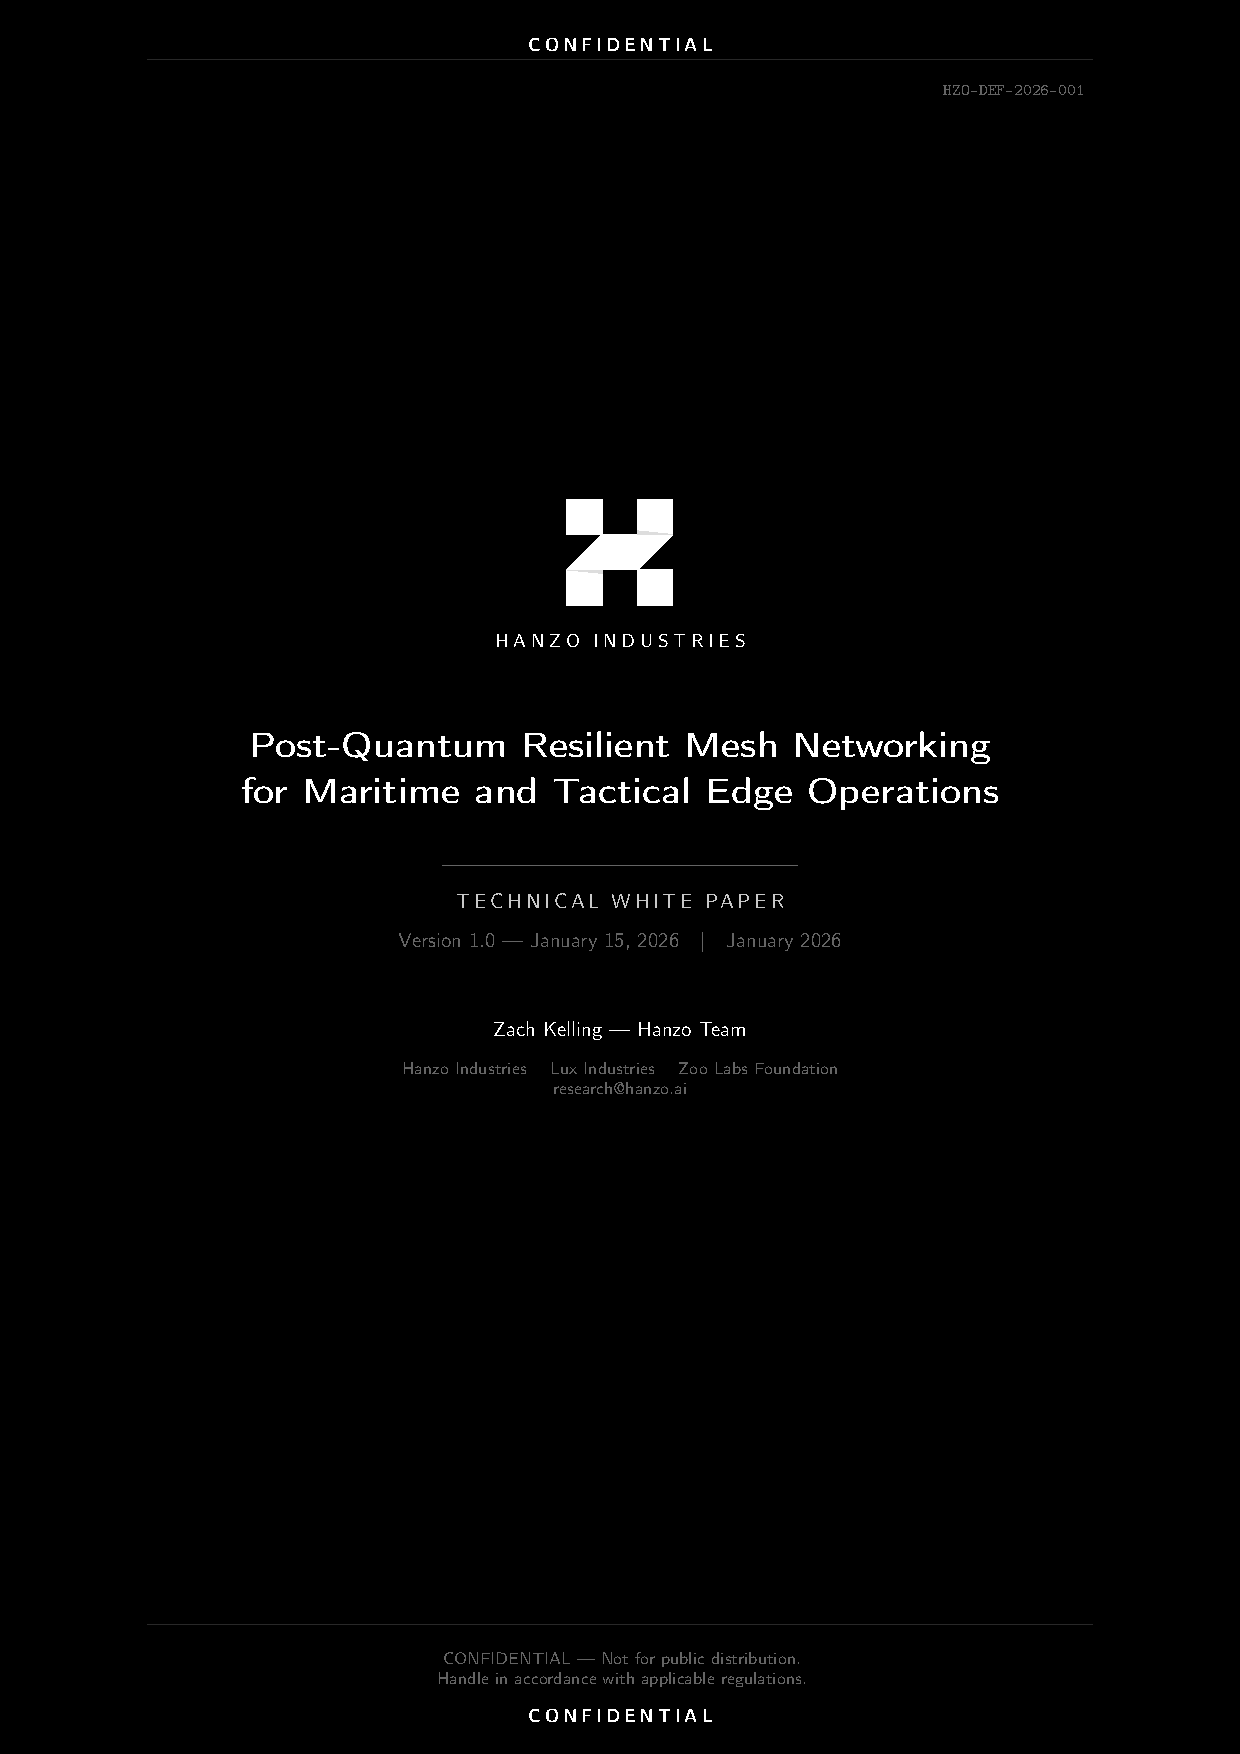
\includepdf[pages=-,fitpaper=true,addtotoc={1,section,0,{Assured Networking},c13}]{hanzo-assured-networking.pdf}

\includepdf[pages=-,fitpaper=true,addtotoc={1,section,0,{Counter-Exploitation},c14}]{hanzo-countermeasures.pdf}

\includepdf[pages=-,fitpaper=true,addtotoc={1,section,0,{Quantum Sensing and QKD},c15}]{hanzo-quantum-sensing-qkd.pdf}
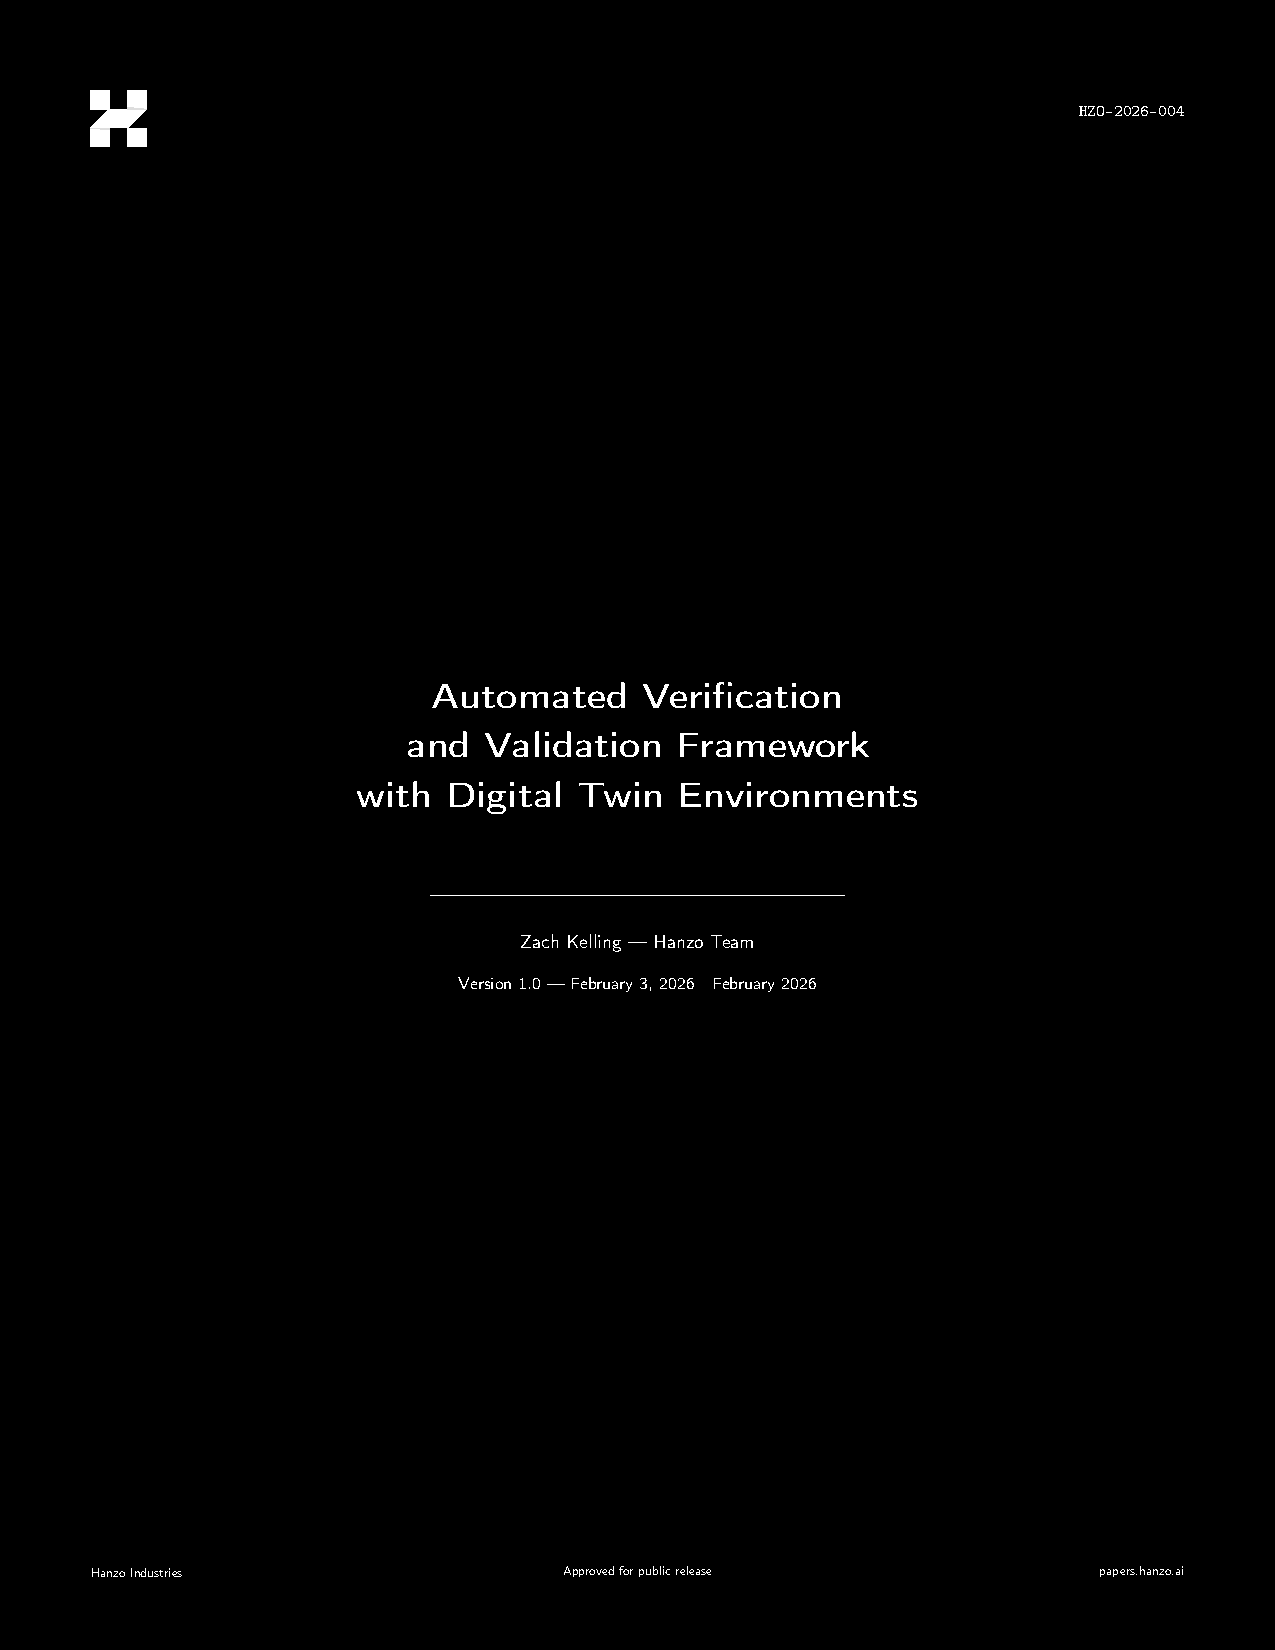
\includepdf[pages=-,fitpaper=true,addtotoc={1,section,0,{Test and Evaluation (V\&V)},c16}]{hanzo-test-evaluation.pdf}

\end{document}
